
%% bare_jrnl.tex
%% V1.3
%% 2007/01/11
%% by Michael Shell
%% see http://www.michaelshell.org/
%% for current contact information.
%%
%% This is a skeleton file demonstrating the use of IEEEtran.cls
%% (requires IEEEtran.cls version 1.7 or later) with an IEEE journal paper.
%%
%% Support sites:
%% http://www.michaelshell.org/tex/ieeetran/
%% http://www.ctan.org/tex-archive/macros/latex/contrib/IEEEtran/
%% and
%% http://www.ieee.org/



% *** Authors should verify (and, if needed, correct) their LaTeX system  ***
% *** with the testflow diagnostic prior to trusting their LaTeX platform ***
% *** with production work. IEEE's font choices can trigger bugs that do  ***
% *** not appear when using other class files.                            ***
% The testflow support page is at:
% http://www.michaelshell.org/tex/testflow/


%%*************************************************************************
%% Legal Notice:
%% This code is offered as-is without any warranty either expressed or
%% implied; without even the implied warranty of MERCHANTABILITY or
%% FITNESS FOR A PARTICULAR PURPOSE! 
%% User assumes all risk.
%% In no event shall IEEE or any contributor to this code be liable for
%% any damages or losses, including, but not limited to, incidental,
%% consequential, or any other damages, resulting from the use or misuse
%% of any information contained here.
%%
%% All comments are the opinions of their respective authors and are not
%% necessarily endorsed by the IEEE.
%%
%% This work is distributed under the LaTeX Project Public License (LPPL)
%% ( http://www.latex-project.org/ ) version 1.3, and may be freely used,
%% distributed and modified. A copy of the LPPL, version 1.3, is included
%% in the base LaTeX documentation of all distributions of LaTeX released
%% 2003/12/01 or later.
%% Retain all contribution notices and credits.
%% ** Modified files should be clearly indicated as such, including  **
%% ** renaming them and changing author support contact information. **
%%
%% File list of work: IEEEtran.cls, IEEEtran_HOWTO.pdf, bare_adv.tex,
%%                    bare_conf.tex, bare_jrnl.tex, bare_jrnl_compsoc.tex
%%*************************************************************************

% Note that the a4paper option is mainly intended so that authors in
% countries using A4 can easily print to A4 and see how their papers will
% look in print - the typesetting of the document will not typically be
% affected with changes in paper size (but the bottom and side margins will).
% Use the testflow package mentioned above to verify correct handling of
% both paper sizes by the user's LaTeX system.
%
% Also note that the "draftcls" or "draftclsnofoot", not "draft", option
% should be used if it is desired that the figures are to be displayed in
% draft mode.
%
\documentclass[journal]{IEEEtran}
\usepackage{blindtext}
\usepackage{graphicx}

% Some very useful LaTeX packages include:
% (uncomment the ones you want to load)


% *** MISC UTILITY PACKAGES ***
%
%\usepackage{ifpdf}
% Heiko Oberdiek's ifpdf.sty is very useful if you need conditional
% compilation based on whether the output is pdf or dvi.
% usage:
% \ifpdf
%   % pdf code
% \else
%   % dvi code
% \fi
% The latest version of ifpdf.sty can be obtained from:
% http://www.ctan.org/tex-archive/macros/latex/contrib/oberdiek/
% Also, note that IEEEtran.cls V1.7 and later provides a builtin
% \ifCLASSINFOpdf conditional that works the same way.
% When switching from latex to pdflatex and vice-versa, the compiler may
% have to be run twice to clear warning/error messages.






% *** CITATION PACKAGES ***
%
%\usepackage{cite}
% cite.sty was written by Donald Arseneau
% V1.6 and later of IEEEtran pre-defines the format of the cite.sty package
% \cite{} output to follow that of IEEE. Loading the cite package will
% result in citation numbers being automatically sorted and properly
% "compressed/ranged". e.g., [1], [9], [2], [7], [5], [6] without using
% cite.sty will become [1], [2], [5]--[7], [9] using cite.sty. cite.sty's
% \cite will automatically add leading space, if needed. Use cite.sty's
% noadjust option (cite.sty V3.8 and later) if you want to turn this off.
% cite.sty is already installed on most LaTeX systems. Be sure and use
% version 4.0 (2003-05-27) and later if using hyperref.sty. cite.sty does
% not currently provide for hyperlinked citations.
% The latest version can be obtained at:
% http://www.ctan.org/tex-archive/macros/latex/contrib/cite/
% The documentation is contained in the cite.sty file itself.






% *** GRAPHICS RELATED PACKAGES ***
%
\ifCLASSINFOpdf
  % \usepackage[pdftex]{graphicx}
  % declare the path(s) where your graphic files are
  % \graphicspath{{../pdf/}{../jpeg/}}
  % and their extensions so you won't have to specify these with
  % every instance of \includegraphics
  % \DeclareGraphicsExtensions{.pdf,.jpeg,.png}
\else
  % or other class option (dvipsone, dvipdf, if not using dvips). graphicx
  % will default to the driver specified in the system graphics.cfg if no
  % driver is specified.
  % \usepackage[dvips]{graphicx}
  % declare the path(s) where your graphic files are
  % \graphicspath{{../eps/}}
  % and their extensions so you won't have to specify these with
  % every instance of \includegraphics
  % \DeclareGraphicsExtensions{.eps}
\fi
% graphicx was written by David Carlisle and Sebastian Rahtz. It is
% required if you want graphics, photos, etc. graphicx.sty is already
% installed on most LaTeX systems. The latest version and documentation can
% be obtained at: 
% http://www.ctan.org/tex-archive/macros/latex/required/graphics/
% Another good source of documentation is "Using Imported Graphics in
% LaTeX2e" by Keith Reckdahl which can be found as epslatex.ps or
% epslatex.pdf at: http://www.ctan.org/tex-archive/info/
%
% latex, and pdflatex in dvi mode, support graphics in encapsulated
% postscript (.eps) format. pdflatex in pdf mode supports graphics
% in .pdf, .jpeg, .png and .mps (metapost) formats. Users should ensure
% that all non-photo figures use a vector format (.eps, .pdf, .mps) and
% not a bitmapped formats (.jpeg, .png). IEEE frowns on bitmapped formats
% which can result in "jaggedy"/blurry rendering of lines and letters as
% well as large increases in file sizes.
%
% You can find documentation about the pdfTeX application at:
% http://www.tug.org/applications/pdftex





% *** MATH PACKAGES ***
%
%\usepackage[cmex10]{amsmath}
% A popular package from the American Mathematical Society that provides
% many useful and powerful commands for dealing with mathematics. If using
% it, be sure to load this package with the cmex10 option to ensure that
% only type 1 fonts will utilized at all point sizes. Without this option,
% it is possible that some math symbols, particularly those within
% footnotes, will be rendered in bitmap form which will result in a
% document that can not be IEEE Xplore compliant!
%
% Also, note that the amsmath package sets \interdisplaylinepenalty to 10000
% thus preventing page breaks from occurring within multiline equations. Use:
%\interdisplaylinepenalty=2500
% after loading amsmath to restore such page breaks as IEEEtran.cls normally
% does. amsmath.sty is already installed on most LaTeX systems. The latest
% version and documentation can be obtained at:
% http://www.ctan.org/tex-archive/macros/latex/required/amslatex/math/





% *** SPECIALIZED LIST PACKAGES ***
%
%\usepackage{algorithmic}
% algorithmic.sty was written by Peter Williams and Rogerio Brito.
% This package provides an algorithmic environment fo describing algorithms.
% You can use the algorithmic environment in-text or within a figure
% environment to provide for a floating algorithm. Do NOT use the algorithm
% floating environment provided by algorithm.sty (by the same authors) or
% algorithm2e.sty (by Christophe Fiorio) as IEEE does not use dedicated
% algorithm float types and packages that provide these will not provide
% correct IEEE style captions. The latest version and documentation of
% algorithmic.sty can be obtained at:
% http://www.ctan.org/tex-archive/macros/latex/contrib/algorithms/
% There is also a support site at:
% http://algorithms.berlios.de/index.html
% Also of interest may be the (relatively newer and more customizable)
% algorithmicx.sty package by Szasz Janos:
% http://www.ctan.org/tex-archive/macros/latex/contrib/algorithmicx/




% *** ALIGNMENT PACKAGES ***
%
%\usepackage{array}
% Frank Mittelbach's and David Carlisle's array.sty patches and improves
% the standard LaTeX2e array and tabular environments to provide better
% appearance and additional user controls. As the default LaTeX2e table
% generation code is lacking to the point of almost being broken with
% respect to the quality of the end results, all users are strongly
% advised to use an enhanced (at the very least that provided by array.sty)
% set of table tools. array.sty is already installed on most systems. The
% latest version and documentation can be obtained at:
% http://www.ctan.org/tex-archive/macros/latex/required/tools/


%\usepackage{mdwmath}
%\usepackage{mdwtab}
% Also highly recommended is Mark Wooding's extremely powerful MDW tools,
% especially mdwmath.sty and mdwtab.sty which are used to format equations
% and tables, respectively. The MDWtools set is already installed on most
% LaTeX systems. The lastest version and documentation is available at:
% http://www.ctan.org/tex-archive/macros/latex/contrib/mdwtools/


% IEEEtran contains the IEEEeqnarray family of commands that can be used to
% generate multiline equations as well as matrices, tables, etc., of high
% quality.


%\usepackage{eqparbox}
% Also of notable interest is Scott Pakin's eqparbox package for creating
% (automatically sized) equal width boxes - aka "natural width parboxes".
% Available at:
% http://www.ctan.org/tex-archive/macros/latex/contrib/eqparbox/





% *** SUBFIGURE PACKAGES ***
%\usepackage[tight,footnotesize]{subfigure}
% subfigure.sty was written by Steven Douglas Cochran. This package makes it
% easy to put subfigures in your figures. e.g., "Figure 1a and 1b". For IEEE
% work, it is a good idea to load it with the tight package option to reduce
% the amount of white space around the subfigures. subfigure.sty is already
% installed on most LaTeX systems. The latest version and documentation can
% be obtained at:
% http://www.ctan.org/tex-archive/obsolete/macros/latex/contrib/subfigure/
% subfigure.sty has been superceeded by subfig.sty.



%\usepackage[caption=false]{caption}
%\usepackage[font=footnotesize]{subfig}
% subfig.sty, also written by Steven Douglas Cochran, is the modern
% replacement for subfigure.sty. However, subfig.sty requires and
% automatically loads Axel Sommerfeldt's caption.sty which will override
% IEEEtran.cls handling of captions and this will result in nonIEEE style
% figure/table captions. To prevent this problem, be sure and preload
% caption.sty with its "caption=false" package option. This is will preserve
% IEEEtran.cls handing of captions. Version 1.3 (2005/06/28) and later 
% (recommended due to many improvements over 1.2) of subfig.sty supports
% the caption=false option directly:
%\usepackage[caption=false,font=footnotesize]{subfig}
%
% The latest version and documentation can be obtained at:
% http://www.ctan.org/tex-archive/macros/latex/contrib/subfig/
% The latest version and documentation of caption.sty can be obtained at:
% http://www.ctan.org/tex-archive/macros/latex/contrib/caption/




% *** FLOAT PACKAGES ***
%
%\usepackage{fixltx2e}
% fixltx2e, the successor to the earlier fix2col.sty, was written by
% Frank Mittelbach and David Carlisle. This package corrects a few problems
% in the LaTeX2e kernel, the most notable of which is that in current
% LaTeX2e releases, the ordering of single and double column floats is not
% guaranteed to be preserved. Thus, an unpatched LaTeX2e can allow a
% single column figure to be placed prior to an earlier double column
% figure. The latest version and documentation can be found at:
% http://www.ctan.org/tex-archive/macros/latex/base/



%\usepackage{stfloats}
% stfloats.sty was written by Sigitas Tolusis. This package gives LaTeX2e
% the ability to do double column floats at the bottom of the page as well
% as the top. (e.g., "\begin{figure*}[!b]" is not normally possible in
% LaTeX2e). It also provides a command:
%\fnbelowfloat
% to enable the placement of footnotes below bottom floats (the standard
% LaTeX2e kernel puts them above bottom floats). This is an invasive package
% which rewrites many portions of the LaTeX2e float routines. It may not work
% with other packages that modify the LaTeX2e float routines. The latest
% version and documentation can be obtained at:
% http://www.ctan.org/tex-archive/macros/latex/contrib/sttools/
% Documentation is contained in the stfloats.sty comments as well as in the
% presfull.pdf file. Do not use the stfloats baselinefloat ability as IEEE
% does not allow \baselineskip to stretch. Authors submitting work to the
% IEEE should note that IEEE rarely uses double column equations and
% that authors should try to avoid such use. Do not be tempted to use the
% cuted.sty or midfloat.sty packages (also by Sigitas Tolusis) as IEEE does
% not format its papers in such ways.


%\ifCLASSOPTIONcaptionsoff
%  \usepackage[nomarkers]{endfloat}
% \let\MYoriglatexcaption\caption
% \renewcommand{\caption}[2][\relax]{\MYoriglatexcaption[#2]{#2}}
%\fi
% endfloat.sty was written by James Darrell McCauley and Jeff Goldberg.
% This package may be useful when used in conjunction with IEEEtran.cls'
% captionsoff option. Some IEEE journals/societies require that submissions
% have lists of figures/tables at the end of the paper and that
% figures/tables without any captions are placed on a page by themselves at
% the end of the document. If needed, the draftcls IEEEtran class option or
% \CLASSINPUTbaselinestretch interface can be used to increase the line
% spacing as well. Be sure and use the nomarkers option of endfloat to
% prevent endfloat from "marking" where the figures would have been placed
% in the text. The two hack lines of code above are a slight modification of
% that suggested by in the endfloat docs (section 8.3.1) to ensure that
% the full captions always appear in the list of figures/tables - even if
% the user used the short optional argument of \caption[]{}.
% IEEE papers do not typically make use of \caption[]'s optional argument,
% so this should not be an issue. A similar trick can be used to disable
% captions of packages such as subfig.sty that lack options to turn off
% the subcaptions:
% For subfig.sty:
% \let\MYorigsubfloat\subfloat
% \renewcommand{\subfloat}[2][\relax]{\MYorigsubfloat[]{#2}}
% For subfigure.sty:
% \let\MYorigsubfigure\subfigure
% \renewcommand{\subfigure}[2][\relax]{\MYorigsubfigure[]{#2}}
% However, the above trick will not work if both optional arguments of
% the \subfloat/subfig command are used. Furthermore, there needs to be a
% description of each subfigure *somewhere* and endfloat does not add
% subfigure captions to its list of figures. Thus, the best approach is to
% avoid the use of subfigure captions (many IEEE journals avoid them anyway)
% and instead reference/explain all the subfigures within the main caption.
% The latest version of endfloat.sty and its documentation can obtained at:
% http://www.ctan.org/tex-archive/macros/latex/contrib/endfloat/
%
% The IEEEtran \ifCLASSOPTIONcaptionsoff conditional can also be used
% later in the document, say, to conditionally put the References on a 
% page by themselves.





% *** PDF, URL AND HYPERLINK PACKAGES ***
%
%\usepackage{url}
% url.sty was written by Donald Arseneau. It provides better support for
% handling and breaking URLs. url.sty is already installed on most LaTeX
% systems. The latest version can be obtained at:
% http://www.ctan.org/tex-archive/macros/latex/contrib/misc/
% Read the url.sty source comments for usage information. Basically,
% \url{my_url_here}.

% *** Do not adjust lengths that control margins, column widths, etc. ***
% *** Do not use packages that alter fonts (such as pslatex).         ***
% There should be no need to do such things with IEEEtran.cls V1.6 and later.
% (Unless specifically asked to do so by the journal or conference you plan
% to submit to, of course. )

\usepackage{amsfonts}
\usepackage{amsmath}
\usepackage{amsthm}
\usepackage{float}
\usepackage{graphicx}
\usepackage{hyperref}
 
\newtheorem{theorem}{Theorem}[section]
\newtheorem{corollary}{Corollary}[theorem]
\newtheorem{lemma}[theorem]{Lemma}

% correct bad hyphenation here
\begin{document}
\title{Upon the Deanonymization of Bitcoin Transactions}
\author{Yash Patel, Matt Weinberg}

\markboth{MAT Senior Thesis 2018}%
{Shell \MakeLowercase{\textit{et al.}}: Bare Demo of IEEEtran.cls for Journals}
\maketitle

\begin{abstract}
\end{abstract}

\section{Introduction}
Bitcoin (BTC), previously relegated as a technology residing in the niche of only the most technologically competent of computer scientists, has emerged into the mainstream public in an enormous way. Ever since its explosive rise over the past year, technologists and investors both have sought to understand and exploit its technical limits. As illustrated in Figure \ref{fig:BTC_price}, speculation on the asset of Bitcoin has become an undeniable sector of the modern technology world, especially when viewed from those outside of it. While current speculations are high, many investors and technologists both struggle to understand the fundamental use case of Bitcoin and its underlying technology: blockchain. The speculative bubble is largely the product of vacuous interest pooling into an asset of misunderstood potential, paralleling the financial bubble surrounding the dot-com bubble. 

\begin{figure}
    \label{fig:BTC_price}
    \centering
    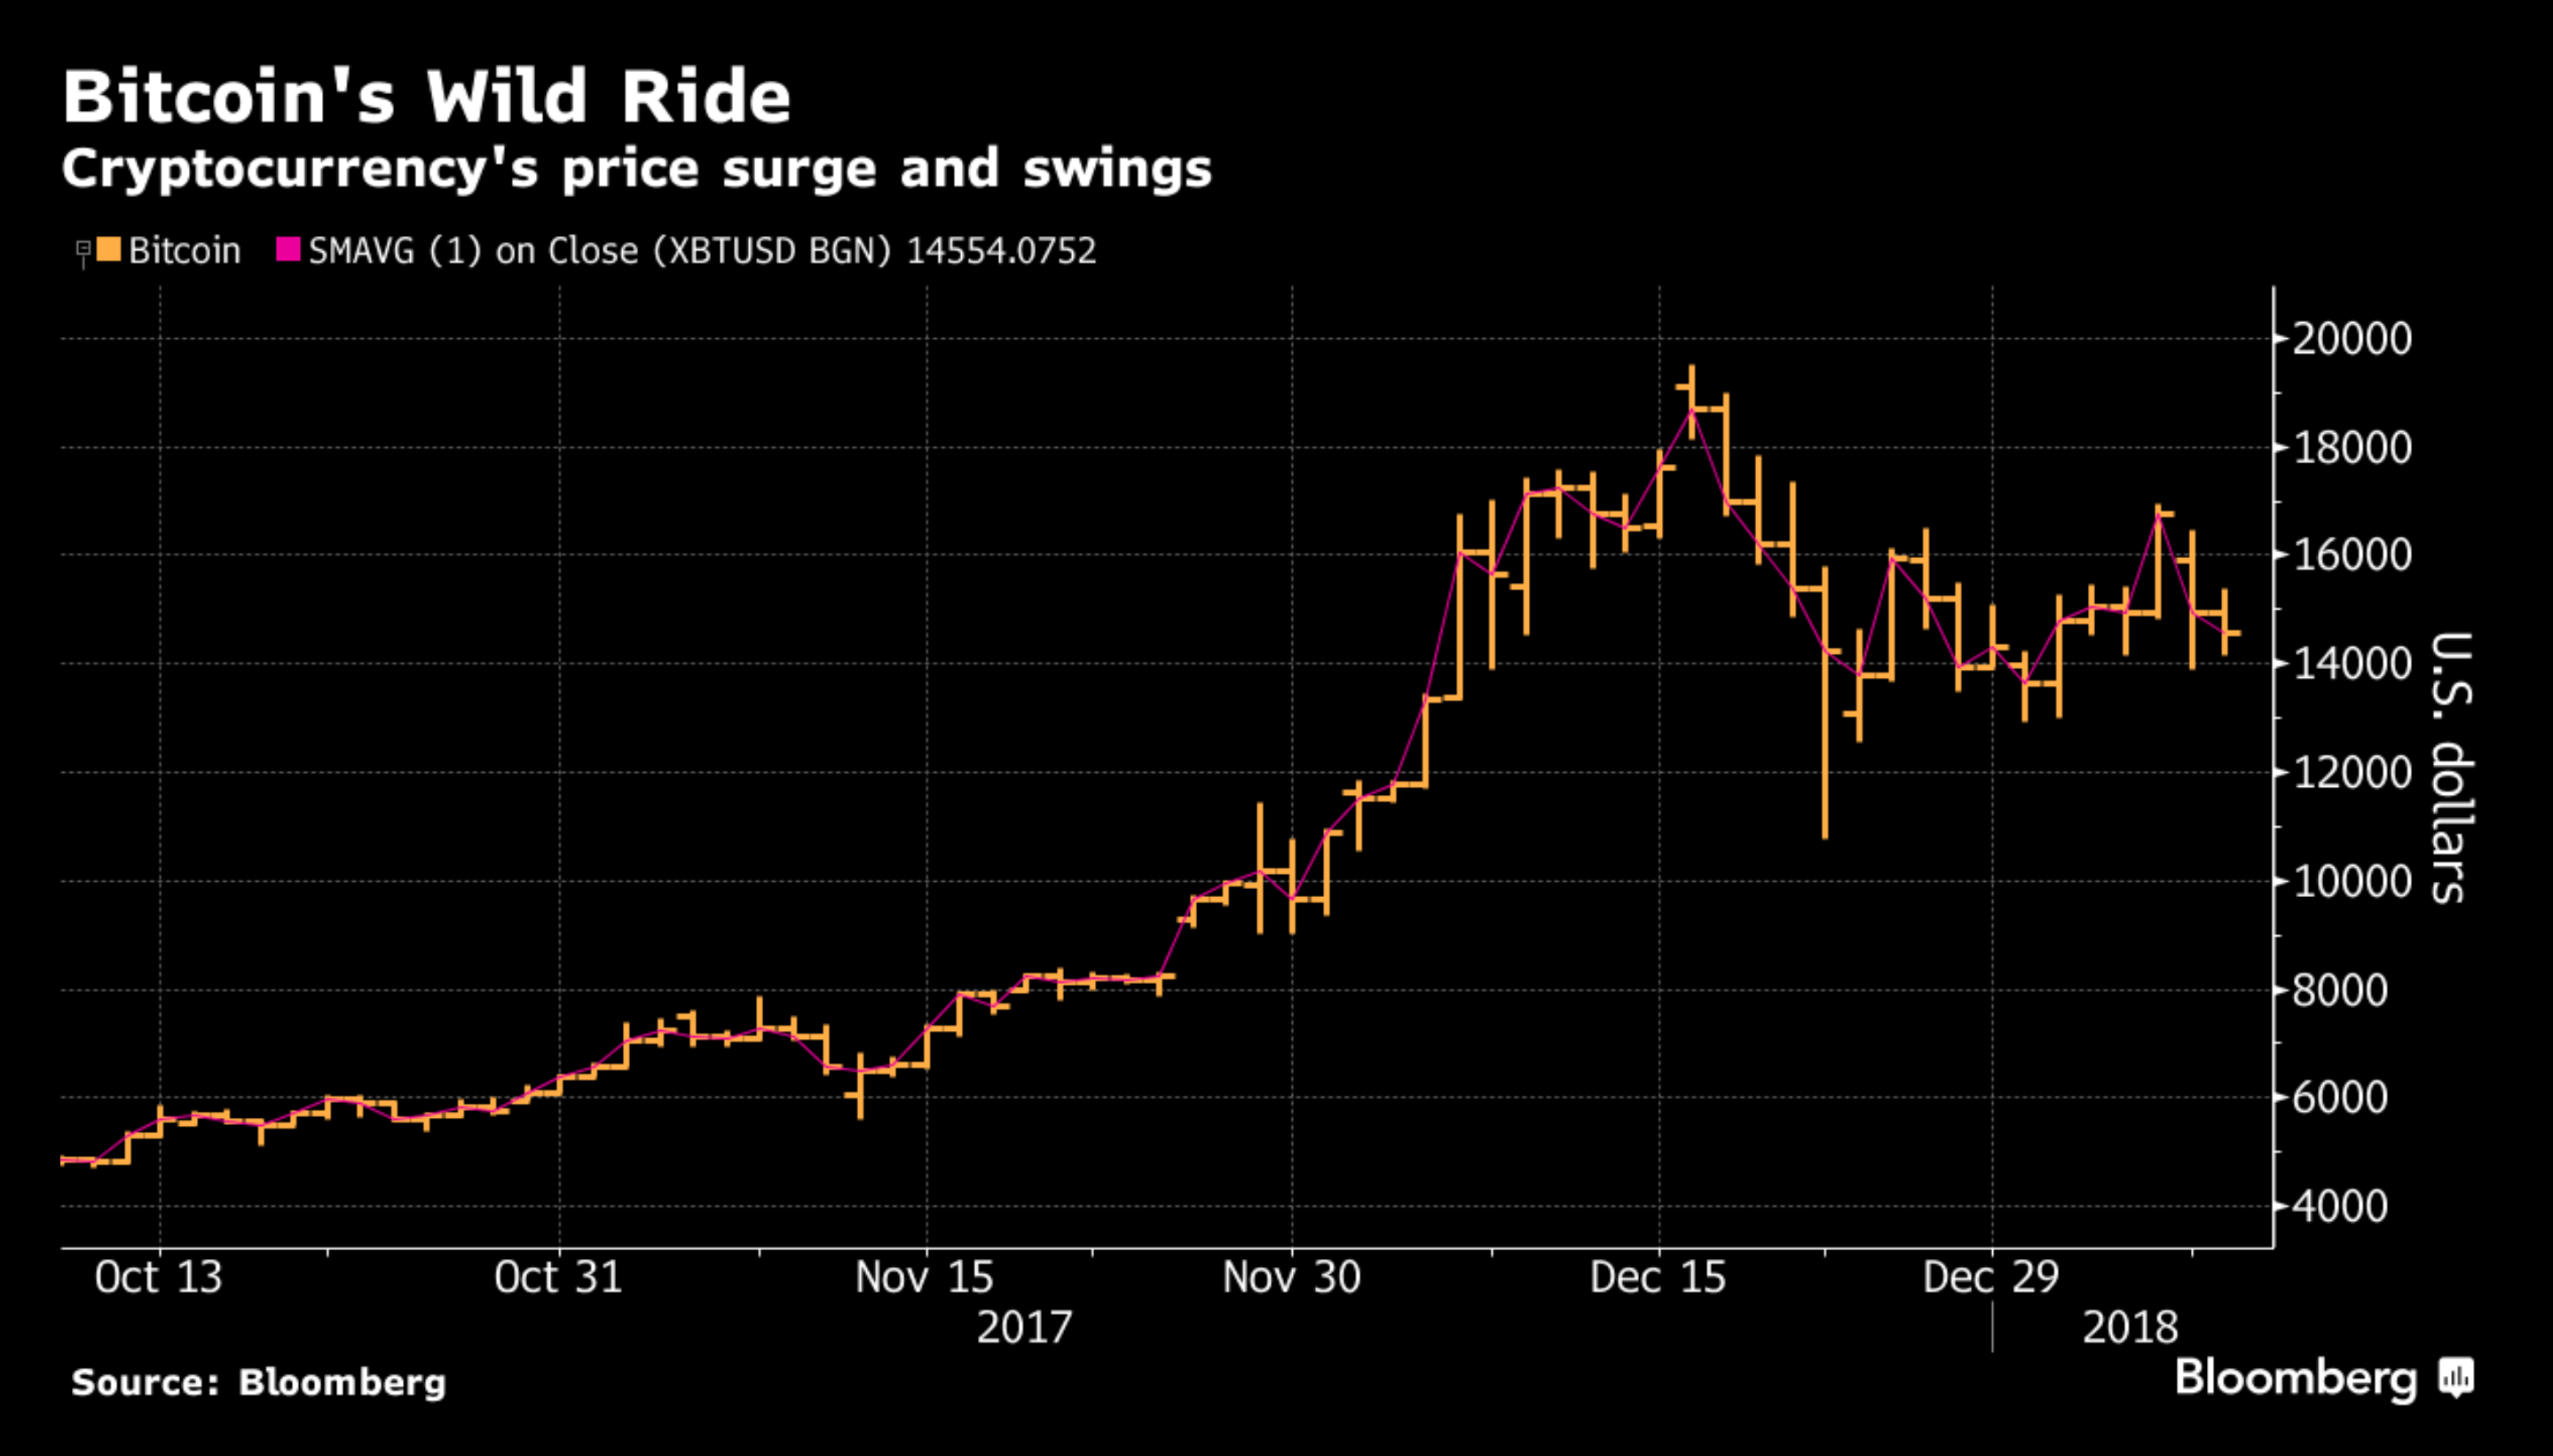
\includegraphics[width=0.4\textwidth]{BTC_price.png}
    \caption{The price of one Bitcoin, as marked by Bloomberg. While technologists saw its promise many years prior, Bitcoin's rise in popularity in the general public has led to exponential speculative interest \cite{goldman}.}
\end{figure}

Prior to further discussing Bitcoin's use cases as a whole, it serves a purpose to understand both the technology and underlying technology first. Briefly, Bitcoin is a cryptocurrency, by which we mean a ``digital unit of exchange that is not backed by a government-issued legal tender" \cite{virtual}. The blockchain technology underpinning Bitcoin and other cryptocurrencies, as illustrated in Figure \ref{fig:blockchain}, is ``a solution to the double-spending problem using a peer-to-peer distributed timestamp server to generate computational proof of the chronological order of transactions. The system is secure as long as honest nodes collectively control more CPU power than any cooperating group of attacker nodes" \cite{bitcoin}. Described plainly, blockchain seeks to solve a technical problem, namely that of achieving consensus in a distributed system while preventing double-spending of the asset being exchanged, i.e. arbitrating exchange of a common asset without the need of a trusted central authority. Since the desired end goal is transactions without a trusted third-party, it must be the case that any peer in this network can verify transactions as valid, which has a natural correspondence to the well-known concept of public-key encryption. It, therefore, should come as little surprise that this is how wallets are implemented in Bitcoin and similar cryptocurrencies.

Specifically, as with any public-key encryption system, Bitcoin exchange revolves around participating members having two keys, one public and one private. For the specific use case of Bitcoin, the private key is used to sign any transactions messages from one account to another. In turn, any other account, particularly that of a receiving party, can verify it indeed originated from the claimed party using the public key, as demonstrated in further detail in Figure \ref{fig:}.

\begin{figure}
    \label{fig:address}
    \centering
    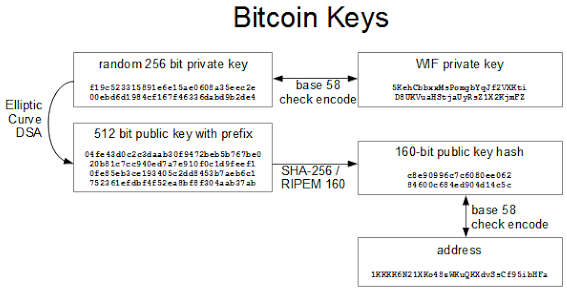
\includegraphics[width=0.4\textwidth]{address.png}
    \caption{While public-key encryption is the basic idea behind the Bitcoin protocol, there are many additional details involved in making it a practical system to be used. In particular, many additional hashing functions are used in an effort to making the underlying key hashes more manageable to deal with and store, while meeting sufficient security demands. These details, while interesting in their own right, however, are not of key important for this particular study \cite{public-key}.}
\end{figure}

Incidentally, these public keys serve as what people colloquially refer to as ``wallet." Specifically, ``Bitcoin, by contrast, is designed with pseudonymous identities. Account numbers are public keys of a specific asymmetric encryption system" \cite{laundering}. This notion of Bitcoin being ``pseudonymous" simply refers to the presence of an abstraction layer between real life and those IDs used within the Bitcoin universe.

\begin{figure}
    \label{fig:blockchain}
    \centering
    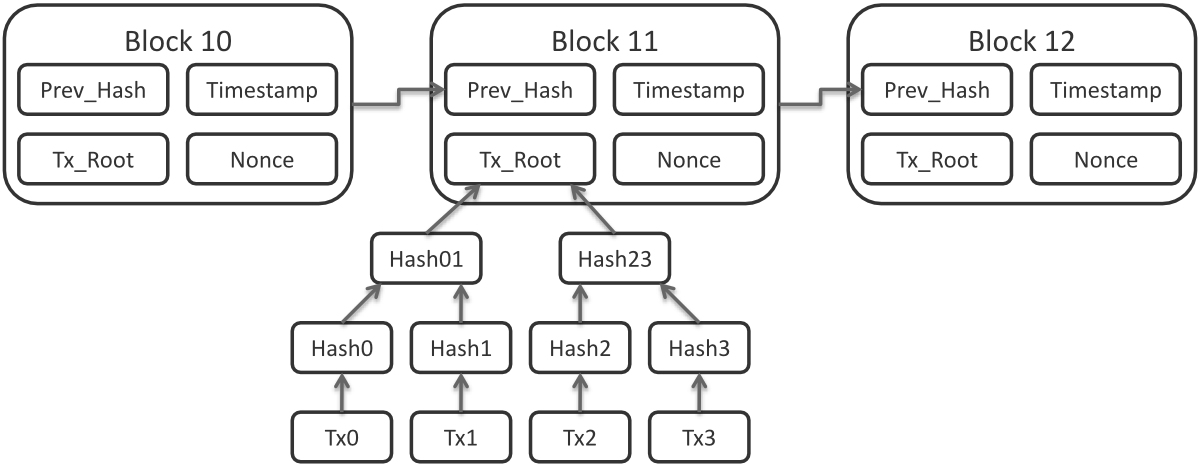
\includegraphics[width=0.4\textwidth]{blockchain.png}
    \caption{Blockchain, the underlying technology behind Bitcoin and all other cryptocurrencies, is simply a data structure consisting of an extended linked list of hash pointers with metadata. These pieces of metadata, in addition to carrying the actual BTC information of interest, more importantly serve as a piece of data that can be used for efficient verification of double-spending in a distributed system \cite{blockchain-img}.}
\end{figure}

Returning to the discussion of interest, Bitcoin when viewed from this perspective has nothing inherently making it more adept with privacy aside from the abstraction of people to public wallet addresses. Yet, this is seemingly fully comparable to the abstraction imposed by the current banking system of the abstraction between a person's account/routing number and real life identity. The key differences, however, are twofold. In the first place, the abstraction layer instituted by banks are leaky. That is to say, while people generally do not know one another banking numbers, authorities within banks have this association, for they oftentimes require personal details be provided in signing up for a bank account. Bitcoin has no similar gatekeeper with such identifying information by virtue of creating a authority-free protocol, meaning Bitcoin wallets can be procured without the need to link it with personal details. The second distinguishing feature is the ease with which such wallets can be created. In line with the lack of a central authority, there is no barrier in place preventing a single person or entity from creating many Bitcoin wallets. This follows as, in the process of making a wallet, there is \textit{no} way to distinguish whether the creator is someone who has made a wallet or not by the lack of associated identifying attributes. Thus, the properties of privacy that have come to be associated with Bitcoin have been born out of its lack of a central authority holding identifying links. 

Returning to the discussion of the use cases of Bitcoin, many have been born out of this seeming impossibility in linking real-life identity with associated transaction wallets. It, therefore, seems natural that such use cases are generally of some illicit nature, as, if they were not, there would be no benefit of using Bitcoin over a traditional bank, as the former does not provide the typical fraud protections that are instituted by the latter. One government report discussed cryptocurrencies in the following light:

``[Cryptocurrencies] present particularly difficult law enforcement challenges because of their ability to transcend national borders in the fraction of a second, unique jurisdictional issues and anonymity due to encryption. Due primarily to their anonymity, virtual currencies have been linked to numerous types of crimes, including facilitating marketplaces for: assassins, attacks on businesses, the exploitation of children (including pornography), corporate espionage, counterfeit currencies, drugs, fake IDs and passports, high yield investment schemes (Ponzi schemes and other financial frauds), sexual exploitation, stolen credit cards and credit card numbers, and weapons" \cite{virtual-currency}. 

To point to one particular example, the Silk Road, an ``online market...[that] specialized in `black market' goods, such as pornography, weapons or narcotics...corresponded to about 4.5\% of all transactions occurring in exchange" during the early days of Bitcoin \cite{silk}. While Bitcoin's integration into the mainstream has greatly exploded since these statistics were measured, the fact remains that a significant portion of Bitcoin's trading activity lie in either illicit or speculation markets. It, therefore, becomes a question of interest whether such illicit activity can be tracked and retraced. By this, we mean to say, produce a map that links wallet addresses to real-life identities. What is meant by ``real-life identities" is somewhat ill-defined, as to what level of granularity we wish to resolve. For example, a group of addresses could be resolved as ``John Smith" or ``Coinbase" assuming John Smith has his wallet handled through Coinbase. Briefly, Coinbase performs two primary purposes: serving as a platform of exchange for cryptocurrencies and providing a simply way to set up corresponding wallets. These wallets, however, are not ``owned" by the end user in the traditional sense, since the private key is owned by Coinbase. Internally, they simply have a map linking a particular private key to the user's account meaning any activity performed by the user on Coinbase is simply relayed to the Coinbase API, which serves as a ``middleman" to the end Bitcoin application layer. The main relevant information is that Coinbase serves as a centarl manager of the accounts of many end users, making it a clear target for deanonymization, as we further expound upon in Section \ref{background}.

Thus, the main objective of the study herein is to deanonymize Bitcoin transacations to as great an extent as possible, as expounded upon above. The outline of this paper is as follows:
\begin{itemize}
    \item Section \ref{background}: Covers through the major technical topics of interest that are to be used in the remainder of the paper. Most of the findings presented through this section entail a literature review of well-known works in their respective fields, although occasional novel material is presented when appropriate for sake of organization. We further note that a majority of figures presented through this section entail those catered from previous research endeavors.
    \item Section \ref{methodology}: Walks through the structure of the experiments that were written and conducted. The code is freely available at: \url{https://github.com/yashpatel5400/anonychain}. We further provide the specifics of the expected structure of results from each experiment.
    \item Section \ref{results}: Presents the results of the experiments laid of in the previous section, largely in the form of graphs when appropriate and tables otherwise.
    \item Section \ref{discussion}: Discusses the main takeaways from the graphical results as they relate to the research problem posed above. Specifically, these discussions will pointedly answer the extent to which spectral clustering can be used for deanonymizing Bitcoin transactions.
    \item Section \ref{conclusion}: Provide follow-up research ideas that could be pursued should readers feel inspired and interested in furthering the research conducted herein.
\end{itemize}

\section{Background}\label{background}
To follow is the necessary technical background for the paper, of which a majority concentrates on material from graph theory. We begin by presenting the current state-of-the-art in this deanonymization space and subsequently discuss all relevant technical concepts as they relate to this study. 

\subsection{Notation}
Prior to delving into the material itself, we present a comprehensive table of the notation for the background sections below in addition to the remainder of the paper. Note that the concepts presented in Table \ref{tab:notation} will be clarified and more greatly discussed in the corresponding background section. Here we assume the standard notation of $G = (V,E)$ to be a graph with vertices $V$ and edges $E$. Such a graph can be assumed to be simple and undirected for the purposes of this paper. The specific graph of relevance will be more thoroughly explained in the methodology, from which the relevance of such assumptions will become clear.

We additionally assume the standard notation of an upper-case letter (i.e. $M$) for a matrix and lower-case (i.e. $v$) for a vector and similarly $\lambda_{i}$ to be the $i^{\text{th}}$ eigenvalue as chosen when the eigenvalues are sorted from lowest to highest (in value, not magnitude).

\begin{table}[]
\centering
\caption{Notation as used in this paper}
\label{tab:notation}
\begin{tabular}{cc}
\textbf{Symbol} & \textbf{Interpretation} \\ \hline
$G$ & Graph \\
$V$ & Vertices of a graph \\
$E$ & Edges of a graph \\
\end{tabular}
\end{table}

\subsection{Deanonymization Techniques}
Currently, two main studies have come to define the space of deanonymization, whose results and limitations we discuss herein. The objective of both was exactly that we have for this study, presented as ``our goal is not to generally deanonymize all Bitcoin users - as the abstract protocol design itself dictates that this should be impossible - but rather to identify certain idioms of use present in concrete Bitcoin network implementations that erode the anonymity of the users who engage in them" \cite{fistful}. In other words, there is no way to go from the raw BTC address information to a real-world identity. However, as with any practical system, there are often leaks in information due to sheer negligence by the end user. This parallels how, despite there being many supposed ``hacks" of Yahoo mail, this has little to do with the encryption of their internal systems, but rather due to the laziness of end users in procuring difficult-to-guess passwords.

In a similar fashion, end users often reveal information intended to be kept private in public channels. For example, people may post their wallet addresses on online forums, from which a link between the address and a real-world entity can be established. By exploiting side-channel leaked information, we can gather a base set of truth regarding who owns a particular wallet, i.e. catering a list saying that address 1Mz7153HMuxXTuR2R1t78mGSdzaAtNbBWX is owned by John Doe and so on. This list, however, will be a very tiny subset of the addresses produced on the BTC network. It is, therefore, the objective herein to expand from this tiny seed of base information to determine the identities of as many other wallets as possible. While seemingly of little use, the purpose of this becomes clear in remembering that many people use multiple BTC wallets. In other words, John Doe, from the previous example, may own three other wallets other than 1Mz7153HMuxXTuR2R1t78mGSdzaAtNbBWX. Having tainted his privacy with this public information leak, it is our objective, therefore, to associate these other three wallet IDs with his name.

Of course, while gathering a comprehensive ground truth is critical for deanonymizing as great a proportion of the network as possible, we similarly consider it successful to cluster a set of wallets as being owned by a single end user. When any one of these wallets has a public side-channel leak in the future, therefore, this information can be retroactively applied onto the clustering, from which a series of other wallets too become revealed. Thus, the act of grouping wallets as being owned by a single entity is effectively the goal of this study, though we use the procured ground truth as a method of verifying accuracy. Once again, the specifics of this procedure will be elaborated in Section \ref{methodology}.

An example as told by them is as follows: ``This clustering allows us to amplify the results of our re-identification attack: if we labeled one public key as belonging to Mt. Gox, we can now transitively taint the entire cluster containing this public key as belonging to Mt. Gox as well" \cite{fistful}. For context, Mt. Gox served a very similar role to that which Coinbase currently fills. 

Returning to the study at hand, it should therefore be clear why they ``consider de-anonymization of Bitcoin addresses as a clustering problem...Bitcoin address clustering is fairly different from classical clustering problems as there is no direct information about the objects' (addresses) such as coordinates or distances. The other peculiarity of the problem is the vastness of the Bitcoin blockchain, which requires designing computationally efficient algorithms for its' clustering" \cite{automatic}. In other words, there are two problems at hand that require solving. The first is determining and procuring a weighted graph with the property that if the edge connecting two vertices $v_{A},v_{B}$ which we denote as $w_{AB}$ satisfies: $w_{AB} > w_{BC}$, there is a higher likelihood that the wallets associated with vertices $A,B$ indeed correspond to the same real-world entity as compared to the likelihood $B,C$ are the same. The second is that of developing or discerning which clustering algorithms that are capable at running at this scale of magnitude with reasonable accuracy and time required.

We begin by discussing the first issue at hand. While it may seem natural to simply make use of the transaction ($tx$) history, seeing as there is a clear canonical mapping from this transaction to a weighted graph, it becomes clear that two accounts having many transactions between them has no bearing on being the same entity. After all, if account $A$ has many transactions with account $B$, there is no reason to believe they correspond to the same \textit{or} different people. To rephrase, we wish to procure a graph that is built atop the raw transactions with a series of heuristics, some of which have arisen from the the paper being discussed.

Prior to discussing this heuristic, we introduce the notion of a change address. ``Change addresses are the mechanism used to give back to the input user in a transaction, as Bitcoins can be divided only by being spent" \cite{fistful}. In other words, the Bitcoin protocol prevents an account that owns 10 BTC from only sending five of its BTC to another account. Instead, the account must spend the entirety of the 10 BTC, with five going to the desired recipient and the other five to a change address owned by the original owner. Having said that, we can discuss the two heuristics used for linking addresses.

\begin{theorem}
``If two (or more) addresses are inputs to the same transaction, they are controlled by the same user; i.e., for any transaction $t$, all $pk\in\text{inputs}(t)$  are controlled by the same user" \cite{fistful}.
\end{theorem}

The main idea behind this is that all the inputs of a given transaction must sign off the transaction with their private key. We assume that end users are not sharing their private keys, for revealing such information essentially gives the receiver full authority of the associated account, in terms of being able to send any BTC held in the account. It, therefore, seems appropriate to assume that end users are not sharing this information. Thus, as \textit{all} input accounts must sign off the transactions, this means all the private keys must be at present simultaneously to validate the transaction, which can only happen if a single real-world entity knows the private keys of all the associated account. This heuristic is likely the most trustworthy of the ones considered, meaning its percent of false positives is extremely low. 

While this is the case, this heuristic is not remotely comprehensive. That is to say, there are \textit{many} more wallets that are owned by the same entity as compared to those that appear together as inputs in a single transaction. Thus, it is of interest to present other heuristics that may have a lower robustness but still contains some information regarding the likelihood of corresponding to the same real-world entity. The second heuristic presented from the paper was as follows:

\begin{theorem}
``The  one-time  change  address  is  controlled  by the same user as the input addresses; i.e., for any transaction $t$,the controller of $\text{inputs}(t)$ also controls the one-time change address $pk \text{outputs}(t)$ (if such an address exists)" \cite{fistful}.
\end{theorem}

In other words, we expect that change addresses, when identifiable as such, are controlled by the originator of the transaction. To identify change addresses, the following intuition was followed: ``Working off the assumption that a change address has only one input (again,  as it is potentially unknown to its owner and is not re-used by the client), we first looked at the outputs of every trans-action. If only one of the outputs met this pattern, then we identified that output as the change address. If, however, multiple outputs had only one input and thus the change address was ambiguous, we did not label any change address for that transaction" \cite{fistful}.

Thus, this paper procured a clustering by directly applying the two heuristics on the raw transaction graph. The paper, however, faced many issues issues related to directly clustering the graph as defined by these two heuristics. The primary of which was ``falsely linking even a small number of change addresses might collapse the entire graph into large `super-clusters' that are not actually controlled by a single user" \cite{fistful}. We, thus, wish to cater heuristics that tend towards favoring false negatives as compared to false positives with the idea that the latter would result in clustering with little sematic value. In fact, the original iteration of their clustering ``ended up with a giant super-cluster containing the public keys of Mt. Gox, Instawallet, BitPay, and Silk Road, among others" \cite{fistful}. It was only after refining the second heuristic that this issue was resolved and there were distinct clusters formed. The result from this investigation is as displayed in Figure \ref{fig:fistful}. 

\begin{figure}
    \label{fig:fistful}
    \centering
    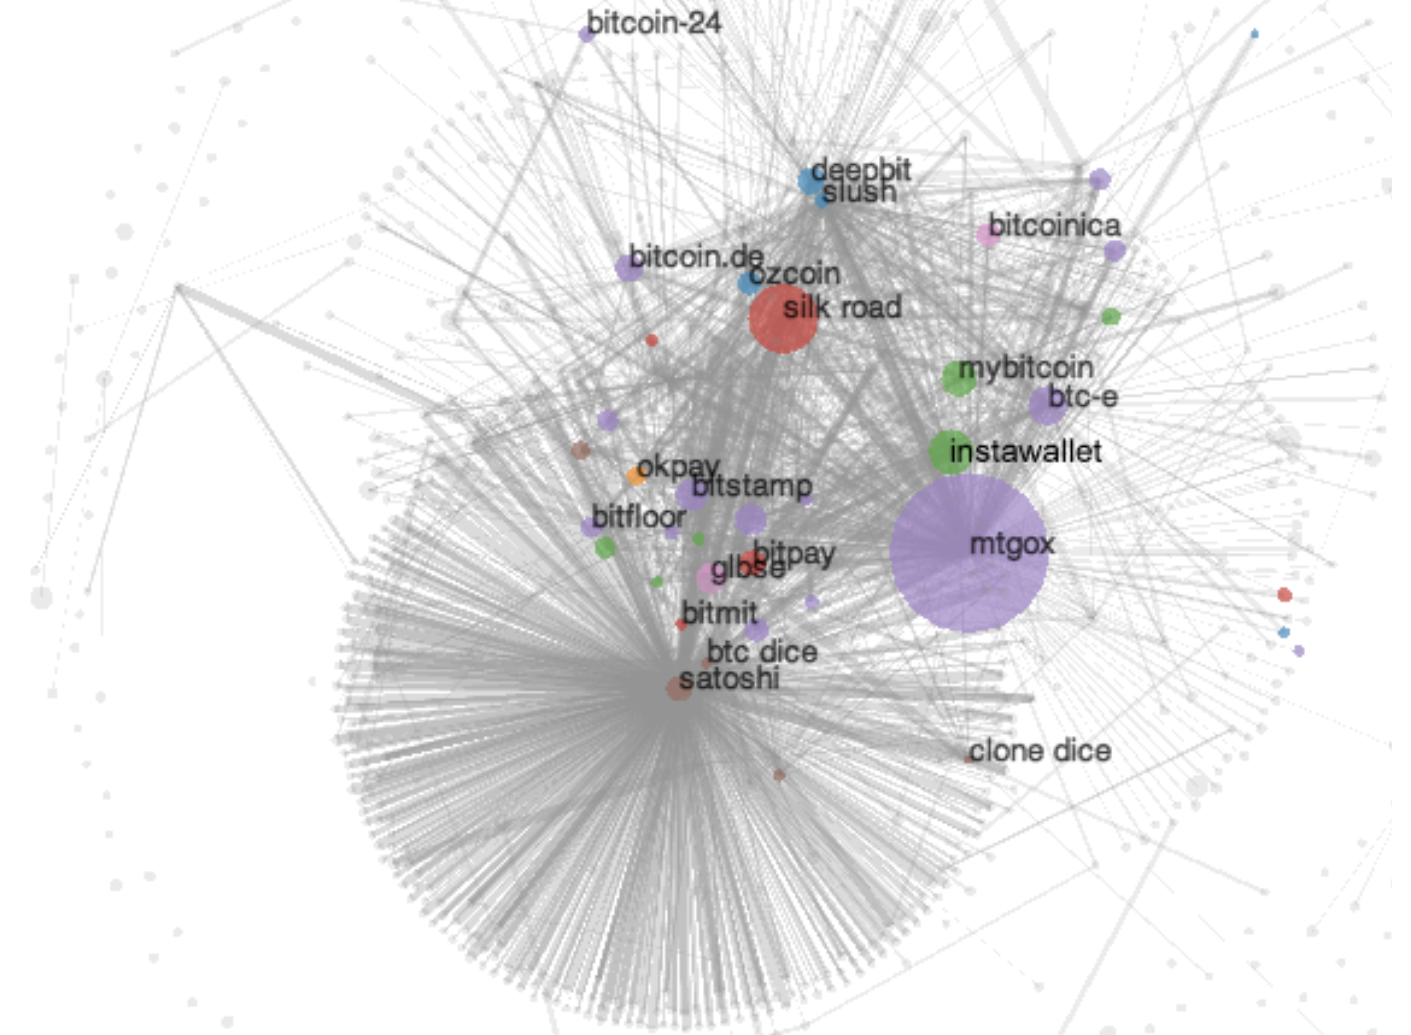
\includegraphics[width=0.4\textwidth]{fistful.png}
    \caption{The deanonymization results from `A Fistful of Bitcoins." This clearly demonstrates that, using careful catered heuristics and large-scale graph clustering, certain portions of the network can be identified with high levels of confidence. The goal of this investigation, therefore, is to procure a graph similar in nature with an even greater number of addresses identified \cite{fistful}.}
\end{figure}

As discussed in the paper itself, there are a few limitations of this investigation, some of which we seek to rectify herein. One such limitation was described as ``given that our new clustering heuristic is not fully robust in the face of changing behavior - how this gap [between actual and potential anonymity] will evolve over time, and what users can do to achieve stronger anonymity guarantee" \cite{fistful}. One key limitation, therefore, is how these two heuristics alone have assumptions that fail to hold under some of the new anonymity services that have emerged atop the BTC network. One such service is called BTC mixing.

These mixing services, also referred to BTC tumblers, effectively mix up the input addresses to a new set of output wallets. In other words, mixing services act as trusted third parties, whereby participating members can transfer their funds to this trusted service wallet, which then distributes the money amongst three new wallets, which then randomly get assigned to the participating members. Of course, the value associated with the accounts involved in the mixing must be sending identical amounts, else the owner of the accounts would be traceable through the mixing service. Assuming no collusion between the owner of the mixing service and any interested third parties, identities cannot be linked between the input and output addresses. The heuristics catered and discussed above, therefore, are unable to link addresses that have passed through such mixing services, since no two such addresses would appear in any connected transaction. This follows as it was the end user's intention in using the mixing service to disassociate the output from the input address, making it highly unlike the two would ever appear concurrently in the future.

While this is the case, assuming the end user has some static characteristics, such as making transactions at only certain times of day or to only particular accounts, the original and mixed addresses should still be linkable, marking a clear deficiency in the heuristics catered above. We, therefore, seek to integrate a broader scope of heuristics to produce potential links between accounts. Of course, with this rising set of heuristics arises the issue brought up within the Fistful of Bitcoins paper, namely that of procuring a series of false positive that ultimately collapse the overall graph into a small number of superclusters. We delve further in depth as to particular methods employed to avoid said issue, but the main workaround deals with another shortcoming of the approach employed by their clustering effort.

In particular, the heuristics they catered were rigidly employed, meaning their involvement in clustering was completely binary. That is to say, if heuristic 1 was satisfied for a pair of vertices, the two were clumped together as being the same entity immediately and similarly for heuristic 2. This rigidness was the source of the collapse and need to make refinements on the second heuristic. We wish to produce a means by which the heuristics can be procured and make the system flexible to the extent that it can automatically determine how effective the different heuristics are at linking two real-world entities and assigning appropriate weights to such heuristics. That is to say, rather than having a binary means of clustering addresses, we wish to expand to a continuous space. 

The second main investigation in the realm of deanonymization, in fact, attempts to do work along these lines. It specifically produces a probabilistic model that attempts to describe the probability two vertices in their graph correspond to the same real-world entity, where the graph contains data both from the on-chain heuristics and off-chain information. Examples of the latter are metadata associated with accounts of a particular entity, that may be used solely \textit{for} the purpose of identification, making it key in procuring a ground truth set. For example, ``Satoshi Bones Casino uses 1change and 1bones prefixes and BTC-E exchange uses 1eEUR and 1eUSD prefixes" \cite{automatic}. With the addition of this additional metadata ``heuristic," however, came additional noise in the sense that there are plenty examples thereof that do not indicate the end-user is in fact the same. As discussed in their paper, ``mostly informationless suffixes  (for example, .com, .co, @gmail)" were ignored \cite{automatic}. 

Towards that end, unlike the Fistful paper, the authors sought to procure a probabilistic model that effectively weights the different heuristics based on their levels of confidence therein. In their words, their ``proposed  model  is  not  intended  to  capture the probabilistic structure of the real world, but more to give an  approach  for  systematical  study  of  confidence  trade-offs between different sources of information" \cite{automatic}. This is similar in nature to the approach to be employed herein. However, their weights were manually tuned by the researchers such that the eventual collapses aligned with expected ground truths. Our investigation seeks to perform such tuning automatically, in a manner that parallels modern machine learning algorithms, specifically neural networks. In addition, we consider several additional heuristics of the off-chain nature described in their paper.

All in all, the current degree to which deanonymization has been accomplished demonstrates it is in fact a viable route of investigation. Yet, their limitations point to a gap in the heuristics that are being employed the the rigidity with which they are being used in doing clustering, which we seek to alleviate herein.

\subsection{Data Procurement}
As discussed in the previous section, it follows that two pieces of data need be procured for this investigation, the first being the ground truth against which perfomance of the deanonymization can be checked and the second the heuristics graph on which the clustering will be performed. For the purposes of this investigation, the gap laid by the former was filled with the ground truth gratefully provided by the authors of the Fistful of Bitcoins paper. As for the latter, however, a further investigation was conducted, from which a tool dubbed ``Blocksci" was produced. Blocksci was born out of a need to begin performing analysis on the public blockchain data. In their words, ``Bitcoin's blockchain alone is 140 GB as of August 2017, and growing quickly. This data holds the key to measuring the privacy of cryptocurrencies in practice...Blocksci is 15x-600x faster than existing tools [and] comes bundled with analytic modules" \cite{blocksci}. In particular, Blocksci fills the void of being able to iterate through the entire blockchain of transactions, allowing for heuristics to similarly be catered in an effectively online setting. That is to say, unlike heuristics procured in the previous investigations, a heuristic that involves traversing the blockchain could be done in a reasonable timeframe by employing Blocksci. Thus, one of the main bottlenecks in procuring more heuristics was eliminated as a result of the development of Blocksci.

While specific details of its internal implementation are not greatly of relevance to this investigation, we present some to make clear the process by which heuristics are produced. This is more clearly elaborated upon in Figure \ref{fig:blocksci}. Specifically, ``BlockSci's design starts with the observation that blockchains are append-only databases; further, the snapshots used for research are static. Thus, the ACID properties of transactional databases are unnecessary" \cite{blocksci}. In other words, by eliminating the unnecessary portions of database API, they streamlined the interface to end users. 

\begin{figure}
    \label{fig:blocksci}
    \centering
    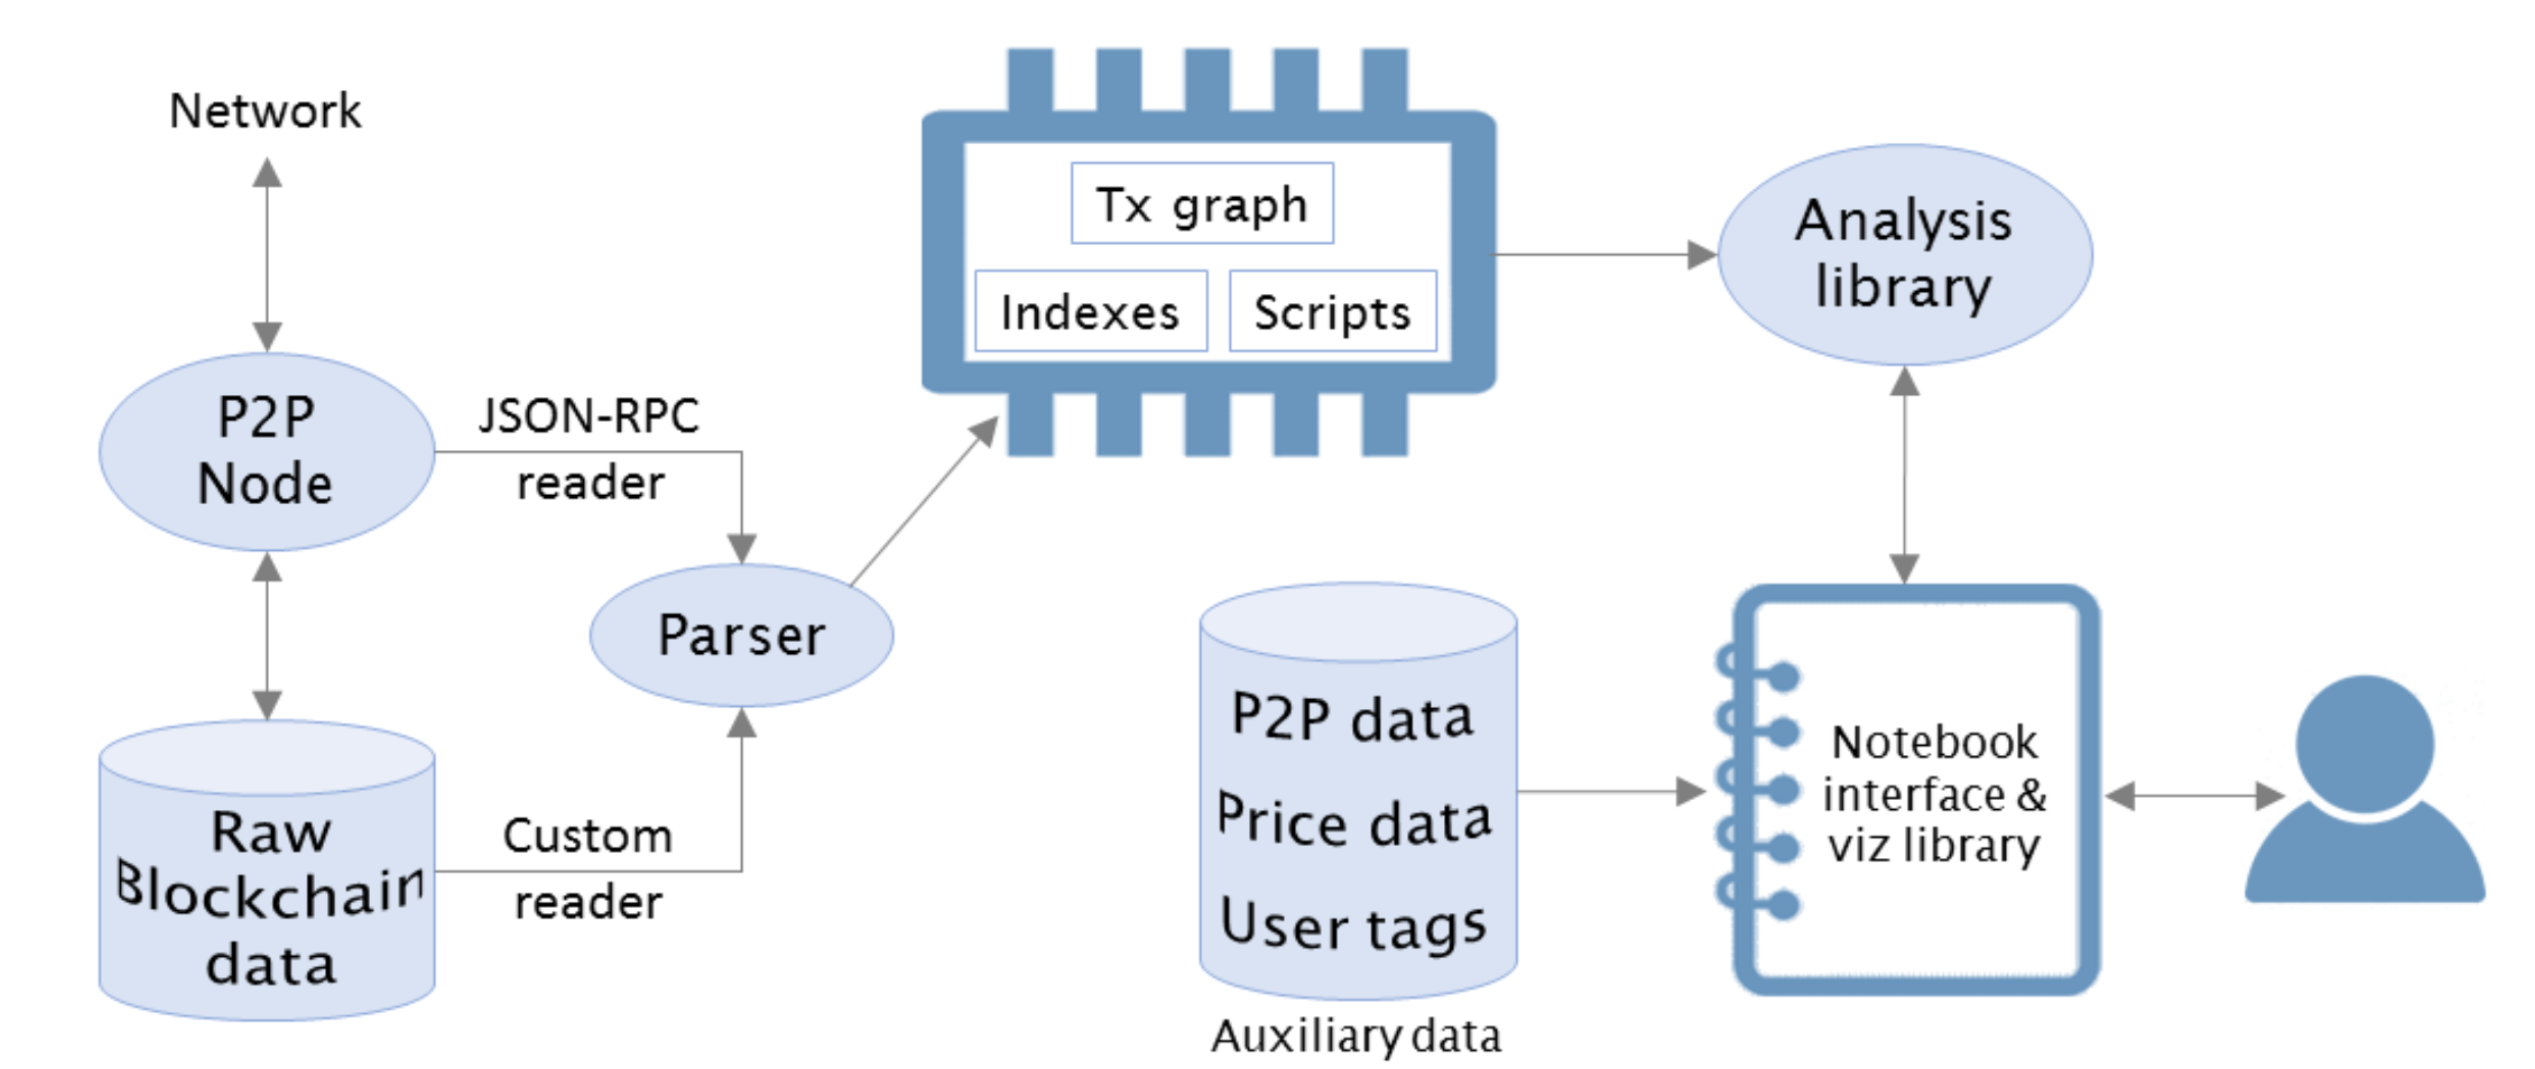
\includegraphics[width=0.4\textwidth]{blocksci.png}
    \caption{The main points of relevance in this figure are the parser and analysis library. As a brief summary, the P2P node refers to the BTC node running on the client, which is constantly getting updates as they are written to blockchain by miners. Thus, the raw blockchain data sitting on the client computer will be parsed and streamlined to produce the optimized iterable data structure, which gets updated as new information arrives from the P2P node. With this iterable struture, an analysis library can be layered atop, to perform work many fold, one example of which is procuring heuristics and performing clustering \cite{blocksci}.}
\end{figure}

In a similar vein, ``The on-disk format of blockchains is highly inefficient for our purposes. It is optimized for a different set of goals such as validating transactions and ensuring immutability...whereas we aim for a single representation of the data that can it in memory" \cite{blocksci}. In other words, the parser for Blocksci implemented many optimizations such that data structures were not as bloated as they are when stored on-disk, as validation was no longer of primary concerning. Using such streamlining and properties of caching, iteration through the blockchain data was, therefore, significantly optimized.

Thus, the main takeway herein was the presence of this additional tool of Blocksci to produce heuristics atop the transactions graph.

\subsection{Overview}
Having established the current state of the art in the deanonymization space, we now turn to presenting the necessary technical background. We begin with an intuition of the layout of the investigation, from which all the pieces to be presented become apparent. Specifically, using the capabilities of Blocksci as elaborated upon above, we procure a set of eight heuristics, about which there are varying degrees of confidence. For sake of completeness, the heuristics are laid out here, as they are presented in \cite{heuristics}:

\begin{itemize}
    \item Sharing inputs in a single transaction
    \item ``If input addresses appear as an output address, the client might have reused addresses for change."
    \item ``If all inputs are of one address type (e.g., P2PKH or P2SH), it is likely that the change output has the same type"
    \item ``Most clients will generate a fresh address for the change. If an output is the first to send value to an address, it is potentially the change."
    \item ``Bitcoin Core sets the locktime to the current block height to prevent fee sniping. If all outpus have been spent, and there is only one output that has been spent in a transaction that matches this transaction’s locktime behavior, it is the change."
    \item ``If there exists an output that is smaller than any of the inputs it is likely the change. If a change output was larger than the smallest input, then the coin selection algorithm wouldn’t need to add the input in the first place."
    \item ``If tx is a peeling chain, returns the smaller output."
    \item ``Detects possible change outputs by checking for output values that are multiples of 10\^digits."
\end{itemize}

With these heuristics, unlike the previous investigations, we do not directly manipulate the original Bitcoin wallet graph. Instead, we procure a \textit{separate} graph, in which nodes correspond to wallet addresses and the edges represent the presence of a heuristic. If multiple heuristics are said to be true between two nodes, the edge connecting said nodes will be the sum of the weights associated with the corresponding heuristics. In other words, denote the weights for these heuristics as $w_1, w_2, ..., w_8$ where $w_i$ naturally takes some weight $\in[0,1]$ corresponding to heuristic $i$. We further assume that these weights are normalized, namely such that $\sum_i w_i = 1$. As an example, if heuristics 2,3, and 4 come up as true between vertices $A,B$, the weight associated with edge $e_{AB}$ will be $w_2+w_3+w_4$.

Upon curating this heuristics graph, we seek to subsequently perform clustering. Unlike the previous investigations, however, there is no rigid binary metric by which we define whether or not two vertices correspond to the same real-world entity. We instead seek to employ standard graph clustering techniques, i.e. k-means, spectral, and DBSCAN, the specifics of which are elaborated upon subsequently in the background. This eventual clustering represents our final result, whose accuracy can be ascertained by comparing whether addresses known to be the same were in fact clustered together or not and vice versa.

\subsection{Stochastic Block Model}
With that being said, this investigation began by modelling the heuristics graph in a simplified light, on which must of the initial experimentation and testing was performed. From here, many optimizations were tested and pruned and different clustering methods evaluated for use on the final dataset. The use case of studying a model rather than the full dataset is twofold. The first is that it allows rapid testing. That is to say, by being able to control exactly the size of the test graphs, many runs could be conducted for a given set of algorithms of interest. In line with that, the second benefit is having a defined metric by which performance could be measured. While there is a subset of known data points in the entire dataset, by having access to the full truth for a simulation, specific pain points could be evaluated. For example, if it turned out a particular algorithm worked well as measured by metric A but not so by metric B but metric A was of greater relevance to the final investigative result, we could easily make use of said algorithm in the final results run. In other words, such experiments made it such that the algorithms' strengths and weaknesses could be understood in great detail, since trials could be procured that targeted different circumstances.

In line with that, we begin our discussion with an introduction to the stochastic block model, commonly shortened to SBM. The SBM is a ``model for random graphs on $n$ nodes with two equal-sized clusters, with an between-class edge probability of $q$ and a within-class edge probability of $p$" \cite{sbm}. We, instead, focus on an expanded view of the SBM. That is to say, rather than solely being between two clusters, we define the SBM to have $n$ clusters such that for any clusters $C_i, C_j$, the probability a vertex in the first will be connected to a vertex in the second is $p$ if $i=j$ and $q$ if $i\neq j$, where $p > q$. In other words, this model produces a random graph comprised of many clusters, of respective sizes $n_1,n_2,...n_k$, with vertices more likely to be connected within a given cluster as compared to other clusters. This, therefore, roughly corresponds to our idealized form of the heuristics graph, namely where the heuristics will be more likely to be present between vertices that belong to the same cluster (i.e. same real-world entity). The main leak in this simplification arises from the fact that, in the case of the SBM, a single run will either have edges or not, with probability $p$ or $q$ depending on the vertices of interest. However, in expectation, namely when average over a series of $n$ runs as $n\rightarrow\infty$, the adjacency matrix will resemble that of the heuristics graph, specifically considering the case where the weights have been normalized, creating a natural correspondence to the probabilities in this matrix:

\[
C=
\left[
\begin{array}{c|c}
M & N \\
\hline
R & S
\end{array}
\right]
\]

The main difference between the two arises in the fact that there is little to suggest different clusters will have similar weights in the heuristics graph. After all, it may be completely obvious that some vertices are in the same clustering, making their associated weight high, while another set of vertices have high uncertainty, making their weight lower, though the two should both be clustered. The natural extension to the SBM would simply having a different $p_i$ for each cluster $C_i$. Yet, this complicates the model to a degree such that the clustering algorithms trials cannot be conducted with the same ease as they could be otherwise. 

As a result, we sacrifice this piece of accuracy with the assumption that algorithm performance on this special case will scale appropriately to the general case. That is to say, we assume that, if algorithm A has better performance on the SBM than B, it should similarly perform better on the generalized case with varying $p_i$, though the two very likely will have degraded performance. The intuition reasoning behind said assumption is that the main detractor of performance will be when there are $p,q$ values that are comparable. Consider the edge case where $p=q$; clearly, this case can have no algorithm that performs clustering with any better accuracy than $50\%$. Thus, the bottleneck of the performance will be the lowest $p_i$ value and similarly the highest $q_{ij}$, where $q_{ij}$ denotes the natural extension of the notion of $q$ to arbitrarily many clusters, namely the probability that a vertex from $C_i,C_j$ will be adjacent. However, we can consider a simulation in which $p,q$ are relatively near one another and evaluate the algorithms' performances on said case. Since this marks the worst/most difficult case, it follows that the best algorithm will similarly scale to be the best in the easier cases. This intuition, however, is confirmed through empirical testing in Section \ref{methodology}.


% Theorem 2.1.Ifa+b>2and(a−b)2≤2(a+b) then, for any fixed vertices uandv , Pn(σu=+SG,σv=+)→12 a.a.s. (8) 

\subsection{Graph Clustering Evaluation}
We further assume that when referring to graph clustering, we wish to separate the set $V$ corresponding to $G$ into sets $\{C_1, C_2, ..., C_n\}$, such that $\cap_{i} C_{i} = \emptyset$, where the objective is to minimize the ``distance" between vertices in a single $C_i$ and maximize that between any $C_i,C_j$ for $i\neq j$, where ``distance" often has a natural interpretation as related to edge weights in the graph.
 
\subsection{Clustering Algorithms}
\subsubsection{K-means}
\subsubsection{Spectral}
\subsubsection{DBSCAN}

\subsection{Matrix Estimation}
\subsection{Online Clustering}
\subsection{Graph Sparsification}
\subsection{Graph Coarsening}

\section{Methodology}\label{methodology}

\section{Results}\label{results}

\section{Discussion}\label{discussion}

\section{Conclusion}\label{conclusion}

\newpage
\begin{thebibliography}{1}
\bibitem{data-stream} Aggarwal, Charu C., et al. ``A Framework for Clustering Evolving Data Streams." Proceedings 2003 VLDB Conference, 2003, pp. 81–92., doi:10.1016/b978-012722442-8/50016-1.
\bibitem{spectral-sparse} Batson, Joshua, et al. ``Spectral Sparsification of Graphs." Communications of the ACM, vol. 56, no. 8, 2013, p. 87., doi:10.1145/2492007.2492029.
\bibitem{coarsening} Chevalier, Cedric, and Ilya Safro. ``Comparison of Coarsening Schemes for Multilevel Graph Partitioning." Lecture Notes in Computer Science Learning and Intelligent Optimization, 2009, pp. 191–205., doi:10.1007/978-3-642-11169-3\_14.
\bibitem{evolutionary-temporal} Chi, Yun, et al. ``Evolutionary Spectral Clustering by Incorporating Temporal Smoothness." Proceedings of the 13th ACM SIGKDD International Conference on Knowledge Discovery and Data Mining - KDD '07, 2007, doi:10.1145/1281192.1281212.
\bibitem{silk} Christin, Nicolas. ``Traveling the Silk Road: A Measurement of a Large Anonymous Online Marketplace." 2012, doi:10.21236/ada579383.
\bibitem{scikit} ``Clustering." Scikit-Learn, scikit-learn.org/stable/modules/clustering.html.
\bibitem{coinjoin} ``CoinJoin: Bitcoin Privacy for the Real World." Bitcoin Talk, 22 Aug. 2013, bitcointalk.org/index.php?topic=279249.0.
\bibitem{dbscan} Daszykowski, M., and B. Walczak. ``Density-Based Clustering Methods." Comprehensive Chemometrics, 2009, pp. 635–654., doi:10.1016/b978-044452701-1.00067-3.
\bibitem{eigen-update} Dhanjal, Charanpal, et al. ``Efficient Eigen-Updating for Spectral Graph Clustering." Neurocomputing, vol. 131, 2014, pp. 440–452., doi:10.1016/j.neucom.2013.11.015.
\bibitem{automatic} Ermilov, Dmitry, et al. ``Automatic Bitcoin Address Clustering." 2017 16th IEEE International Conference on Machine Learning and Applications (ICMLA), 2017, doi:10.1109/icmla.2017.0-118.
\bibitem{evaluation} ``Evaluation of Clustering." Stanford NLP, 2008, nlp.stanford.edu/IR-book/html/htmledition/evaluation-of-clustering-1.html.
\bibitem{follow} Greenberg, Andy. ``Follow The Bitcoins: How We Got Busted Buying Drugs On Silk Road's Black Market." Forbes, Forbes Magazine, 7 Sept. 2013, www.forbes.com/sites/andygreenberg/2013/09/05/follow-the-bitcoins-how-we-got-busted-buying-drugs-on-silk-roads-black-market/\#79bb83c8adf7.
\bibitem{heuristics} ``Heuristics." \textit{BlockSci 0.4.5 Documentation}, citp.github.io/BlockSci/heuristics/heuristics.html. 
\bibitem{blocksci} Kalodner, Harry. ``BlockSci: Design and Applications of a Blockchain Analysis Platform." ArXiv Preprint, 2017, doi:1709.02489.
\bibitem{metis} Karypis, George, and Vipin Kumar. ``METIS--Unstructured Graph Partitioning and Sparse Matrix Ordering System, Version 2.0." 1995.
\bibitem{goldman} Katz, Lily. ``Goldman Says Cryptocurrencies May Succeed as Form of Real Money." Bloomberg.com, Bloomberg, 10 Jan. 2018, www.bloomberg.com/news/articles/2018-01-10/goldman-says-viability-of-crypto-is-highest-in-developing-world.
\bibitem{mincut} Kothari, Pravesh. ``Karger's Min Cut Algorithm." 2015, Princeton University, Princeton University.
\bibitem{dynamic} LaViers, Amy, et al. ``Dynamic Spectral Clustering." Georgia Institute of Technology, 2010.
\bibitem{sketch} Liberty, Edo. ``Simple and Deterministic Matrix Sketching." Proceedings of the 19th ACM SIGKDD International Conference on Knowledge Discovery and Data Mining - KDD '13, 2013, doi:10.1145/2487575.2487623.
\bibitem{spectral} Luxburg, Ulrike Von. ``A Tutorial on Spectral Clustering." Statistics and Computing, vol. 17, no. 4, 2007, pp. 395–416., doi:10.1007/s11222-007-9033-z.
\bibitem{fistful} Meiklejohn, Sarah, et al. ``A Fistful of Bitcoins." Proceedings of the 2013 Conference on Internet Measurement Conference - IMC '13, 2013, doi:10.1145/2504730.2504747.
\bibitem{laundering} Moser, Malte, et al. ``An Inquiry into Money Laundering Tools in the Bitcoin Ecosystem." 2013 APWG ECrime Researchers Summit, 2013, doi:10.1109/ecrs.2013.6805780.
\bibitem{sbm} Mossel, Elchanan, et al. ``Reconstruction and Estimation in the Planted Partition Model." Probability Theory and Related Fields, vol. 162, no. 3-4, 2014, pp. 431–461., doi:10.1007/s00440-014-0576-6.
\bibitem{bitcoin} Nakamoto, Satoshi. ``Bitcoin: A Peer-to-Peer Electronic Cash System." 2008.
\bibitem{incremental} Ning, Huazhong, et al. ``Incremental Spectral Clustering by Efficiently Updating the Eigen-System." Pattern Recognition, vol. 43, no. 1, 2010, pp. 113–127., doi:10.1016/j.patcog.2009.06.001.
\bibitem{dynamic-sbm} Pensky, Marianna, and Teng Zhang. ``Spectral Clustering in the Dynamic Stochastic Block Model." ArXiv Preprint, 2017, doi:1705.01204.
\bibitem{fast-coarsen} Purohit, Manish, et al. ``Fast Influence-Based Coarsening for Large Networks." Proceedings of the 20th ACM SIGKDD International Conference on Knowledge Discovery and Data Mining - KDD '14, 2014, doi:10.1145/2623330.2623701.
\bibitem{spectral-bisection} Rocha, Israel. ``Improvements on Spectral Bisection." ArXiv Preprint, 2017, doi:1703.00268.
\bibitem{cluster-review} Schaeffer, Satu Elisa. ``Graph Clustering." Computer Science Review , 2007, pp. 27–64.
\bibitem{bitcoin-etf} ``Self - Regulatory Organizations; NYSE Arca, Inc; Order Instituting Proceedings to Determine Whether to Approve or Disapprove a Proposed Rule Change to List and Trade the Shares of the ProShares Bitcoin ETF and the ProShares Short Bitcoin ETF under NYSE Arca Rule 8.200 - E, Commentary .02." Securities and Exchange Commission, 23 Mar. 2018.
\bibitem{fast-kmeans} Shindler, Michael, et al. ``Fast and Accurate k-Means For Large Datasets.” Advances in Neural Information Processing Systems, 2011. 
\bibitem{public-key} Shirriff, Ken. ``Ken Shirriff's Blog." Bitcoins the Hard Way: Using the Raw Bitcoin Protocol, www.righto.com/2014/02/bitcoins-hard-way-using-raw-bitcoin.html. 
\bibitem{resistance} Spielman, Daniel A., and Nikhil Srivastava. ``Graph Sparsification by Effective Resistances." Proceedings of the Fourtieth Annual ACM Symposium on Theory of Computing - STOC 08, 2008, doi:10.1145/1374376.1374456.
\bibitem{virtual} Trautman, Lawrence J. ``Virtual Currencies: Bitcoin \& What Now after Liberty Reserve and Silk Road?" SSRN Electronic Journal, 2014, doi:10.2139/ssrn.2393537.
\bibitem{blockchain-img} Wander, Matthaus. ``Bitcoin Block Data." Wikimedia Commons, 22 June 2013, commons.wikimedia.org/wiki/File:Bitcoin\_Block\_Data.png.
\bibitem{scalable} Whang, Joyce Jiyoung, et al. ``Scalable and Memory-Efficient Clustering of Large-Scale Social Networks." 2012 IEEE 12th International Conference on Data Mining, 2012, doi:10.1109/icdm.2012.148.
\bibitem{ico} Zetzsche, Dirk A., et al. ``The ICO Gold Rush: It's a Scam, It's a Bubble, It's a Super Challenge for Regulators." SSRN Electronic Journal, 2017, doi:10.2139/ssrn.3072298.
\end{thebibliography}

\end{document}